Att exekvera ett program symboliskt innebär att representera värden utefter
programflödet som symboliska restriktioner (jfr eng. \emph{constraints}), vilka kan
lösas av automatiserade teoremlösare (\emph{SMT solver}). En symbolisk körning
representerar flera konkreta körningar eftersom de (symboliska) värden som
används representerar grupper av konkreta värden vilka har gemensamt hur de
påverkar programmets flöde~\cite{klee}.

Vägar i programmets kontrollflöde utforskas med symboliska uttryck som kallas
för path constraints (jfr sv.\ vägvillkor) för de begränsningar som finns på
programmets variabler --- vilka egenskaper de måste uppnå för att just denna väg
ska kunna följas~\cite{klee}. Huruvida villkorsblock av program är nårbara kan
evalueras eftersom de krav som måste uppfyllas för att följa vägen dit dokumenteras
under den symboliska körningen, och resulterar i fullständiga symboliska representationer
som en automatiserad teoremlösare (jfr. eng. SMT solver) kan appliceras på.

Eftersom de symboliska värdena har kapacitet att representera grupperingar av konkreta
värden istället för enskilda sådana, utförs en generaliserad testning av programmet,
som ger insikt i hur programmet beter sig givet en grupp av parametrar som alla
på grund av någon eller några gemensamma egenskaper, orsakar gemensamma beteenden
i programmet~\cite{Cadar}.

En symbolisk exekveringsmotor arbetar genom att först representera programmets
indata som symboliska variabler, vilka vid starten inte har några begränsningar.
När programflödet når en branch som baseras på någon av de symboliska
variablerna, väljer motorn en branch och tillsätter dess vägvillkor på den
symboliska variabeln för alla vägar som fortsätter utefter branchen. Operationer
på värden under körningens väg översätts till symboliska operationer på
motsvarande symboliska variabler. När körning utefter branchen är
slutförd repeterar motorn samma metodik på samma branch för att utforska andra
alternativ. De tillståndsvillkor som en viss väg visas ha byggs därför
successivt upp genom att motorn utökar de symboliska variablerna till
villkorliga uttryck allt eftersom vägen följs~\cite{klee}.

Eftersom symbolisk exekvering kan leda till stigexplosionsproblemet, vilket
uppstår i program vars branches växer exponentiellt och resulterar i att en
symbolisk exekvering aldrig terminerar~\cite{path_explo}, är det inte effektivt
att alltid undersöka alla branchar i ett program. Exempel på metoder för att
undvika path explosion är State Merging och heuristik.

För att illustrera symbolisk exekvering används följande pseudokod:

\begin{figure}[H]
    \begin{subfigure}[b]{0.58\textwidth}
        \begin{lstlisting}[language=Python, frame=single,
        basicstyle=\normalfont\ttfamily]
x = input()
y = input()
z = 2 * y

if x == 100000:
  if x < z:
    # fabricated scenario of
    # memory vulnerability
    error_leading_to_mem_vuln()
  else:
    run_other_important_code()
else:
  run_important_code()
\end{lstlisting}
        \caption{} % används för att rendera a) som caption
        \label{fig:symbex_example_code}
    \end{subfigure}
    \begin{subfigure}[t]{0.4\textwidth}
        \centering
        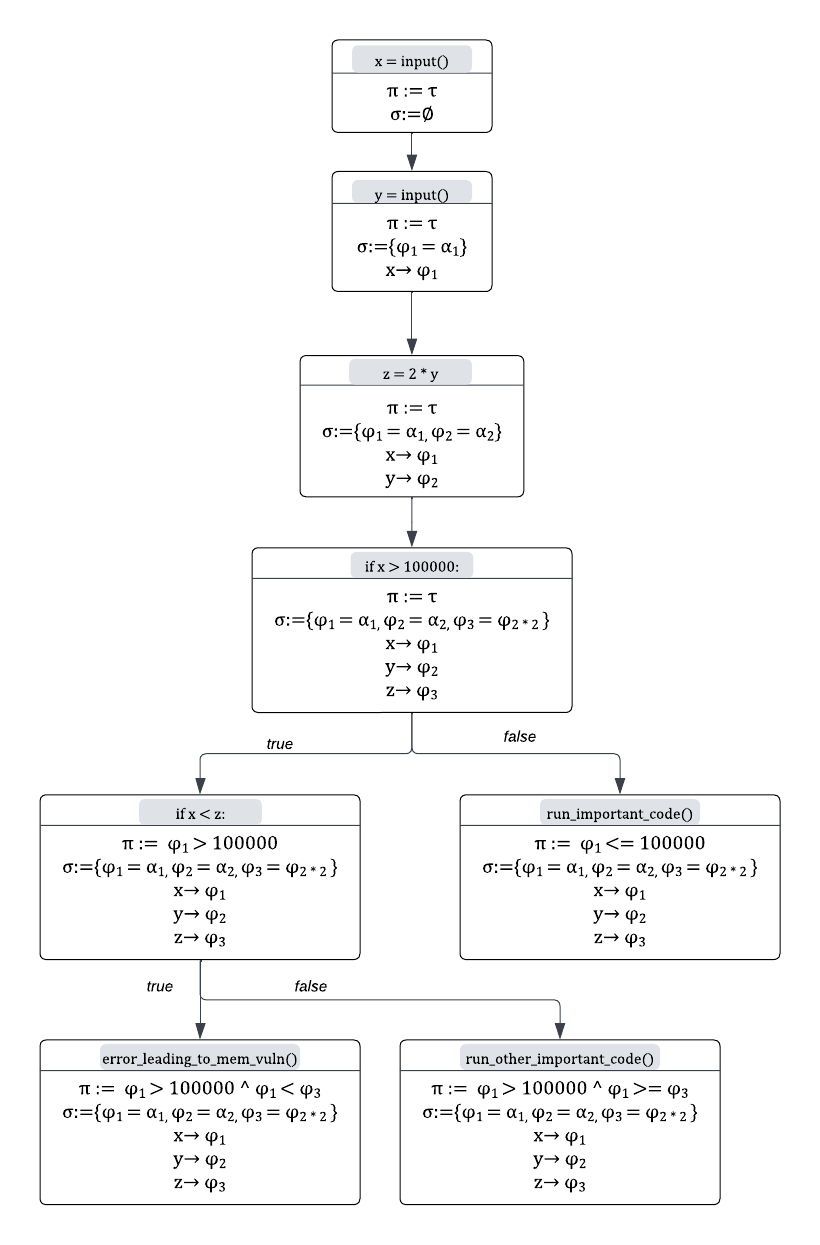
\includegraphics[scale=0.31]{figures/final_symbolic_example_graph.png}
        \caption{} % används för rendera b) som caption
        \label{fig:symbex_example_graph}
    \end{subfigure}

    \caption{Exempel för att visa symbolisk exekvering: pseudokod (a) och path
        constraint och symboliskt tillstånd för alla stigar i pseudokoden angett
        i (b). $  \mathcal{S} = \{\sigma := \{\phi_1 = \alpha_1, \phi_2 = \alpha_2, \phi_3 =
            2\phi_2\}, x \rightarrow \phi_1, y \rightarrow \phi_2, z \rightarrow
            \phi_3\}$}
\end{figure}

Exempelprogrammet i figur~\ref{fig:symbex_example_code} använder symbolisk
exekvering för att hitta vilken indata som leder programexekveringen till de
olika grenarna i programflödet. I många fall är det intressant att göra en
uttömmande sökning och hitta alla möjliga vägar i ett program, något som är
möjligt i detta program men inte alla program. Ett motexempel är komplexa
program som på grund av path explosion inte hittar alla möjliga vägar.
Variablerna \emph{x} och \emph{y} sätts till symboliska värden som sedan används
för att beräkna vägvillkoret och de symboliska uttryck som variablerna utvecklas
till för en vald branch. Därefter används dessa uttryck och path constraint
tillsammans för att bilda en ekvation som kan lösas med hjälp av en SMT-lösare
och därmed få ut ett konkret värde. Figur~\ref{fig:symbex_example_graph} visar
hur det symboliska tillståndet förändras för alla möjliga branches i programmet.

I~\ref{fig:symbex_example_graph} används $\pi$ för att ange vägvillkoret vilket
är initialt satt till $\top$ eftersom villkoret är sant från början och $\sigma$
används för att visa mappningen för symboliska värden. $\pi$ och $\sigma$
populeras längs med exekveringen, och \emph{x} och \emph{y} mappas till
symboliska värden. Beroende på vilken stig som väljs i exekveringen, uppdateras
vägvillkoret. I andra noden sett uppifrån finns det två skillnader i jämförelse
med den första noden: \emph{x} tilldelas $\phi_1$ som är en symbolisk mappning
till $\alpha_1$. Efter den fjärde noden sett uppifrån görs ett val och
vägvillkoret förändras beroende på vilken väg som tas -- vägvillkoret uppdateras
till $\phi_1 > 100000$ om $x < z$ och annars uppdateras det till $\phi_1 <=
    100000$. På samma sätt uppdateras $\pi$ och $\phi$ längs andra exekveringsvägar
och vilket till slut leder till ett komplett programflödesdiagram som beror på
\emph{x, y, z}. I varje nod kan en SMT-lösare appliceras för att ge ett konkret
värde som uppfyller vägvillkoren.
